\paragraph{QuizziPedia::Back-End::App::Models::UserModel}
\label{QuizziPedia::Back-End::App::Models::UserModel}
\begin{figure}[ht]
	\centering
	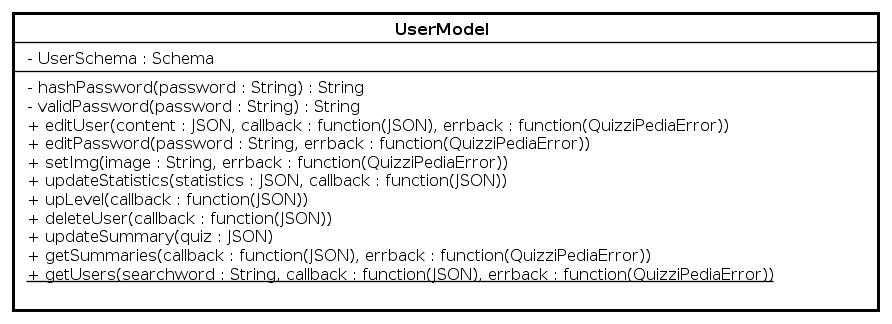
\includegraphics[scale=0.7]{UML/Classi/Back-End/QuizziPedia_Back-End_App_Models_userModel.png}
	\caption{QuizziPedia::Back-End::App::Models::UserModel}
\end{figure}
\FloatBarrier
\begin{itemize}
	\item \textbf{Descrizione}: classe che modella la creazione e la gestione dei dati utente;
	\item \textbf{Utilizzo}: viene utilizzata per rappresentare i dati degli account dei vari utenti dell'applicazione. Si interfaccia alla libreria \textit{Mongoose\ped{G}} per la creazione dello schema e dei relativi metodi statici o di istanza;
	\item \textbf{Relazioni con altre classi}:
		\begin{itemize}
			\item \textbf{IN \textbf {AuthenticationController}} \\
			Classe che si occupa della registrazione e dell'autenticazione dell'utente nel sistema. È un componente ConcreteHandler del design pattern \textit{Chain of responsibility\ped{G}} . Risulta essere il componente che eventualmente esegue la richiesta del client attraverso \textit{Passport\ped{G}};
			\item \textbf{IN \textbf {SessionController} }\\
			Classe \textit{middleware\ped{G}} che, utilizzando \textit{Passport\ped{G}}, si occupa di controllare la consistenza dell'oggetto session durante la sessione associata all’utente autenticato. È un componente ConcreteHandler del design pattern \textit{Chain of responsibility\ped{G}};
			\item \textbf{IN \textbf {UserManagementController}} \\
			Classe che gestisce la logica applicativa riguardante la visualizzazione e la modifica dei dati dell'utente.
Rappresenta il ConcreteHandler nel design pattern \textit{Chain of responsibility\ped{G}}. Utilizza \textit{Passport\ped{G}};
			\textbf{\item OUT \textbf{SummaryModel}} \\
			Questa classe rappresenta il riepilogo dei questionari svolti dagli utenti;
			\textbf{\item IN \textbf{QuestionModel} }\\
			Questa classe rappresenta i dati delle domande create dai vari utenti;
			\textbf{\item IN \textbf{QuizModel}} \\
			Questa classe rappresenta i dati dei questionari creati dagli utenti Pro;
		\end{itemize}
	\item \textbf{Attributi}: 
		\begin{itemize}
			\item \textbf{- \texttt{userSchema}: \texttt{Schema}} \\
			Questo campo dati rappresenta lo schema \textit{Mongoose\ped{G}} dell'utente QuizziPedia. Lo schema prevede i seguenti attributi:
			\begin{itemize}
				\item 
					\texttt{name: String}\\ Rappresenta il nome  dell'utente registrato;
				\item 
					\texttt{surname: String}\\ Rappresenta il cognome  dell'utente registrato;
				\item 
					\texttt{email: String}\\ Rappresenta l'email  dell'utente registrato;
				\item 
					\texttt{userImg: String}\\ Rappresenta il path della foto profilo dell'utente registrato;
				\item 
					\texttt{username: String}\\ Rappresenta l'username con cui viene identificato l'utente all'interno dell'applicazione;		
				\item
					\texttt{password: String}\\ Rappresenta la password associata all'utente,  appositamente codificata mediante l'algoritmo bcrypt;  		
				\item
					\texttt{statistics: Array<Mixed>}\\ Contenente i seguenti attributi:
				\begin{itemize}
					\item
						\texttt{topicName: String}\\ Rappresenta il nome della statistica relativa all'argomento;	 
					\item
						 \texttt{topicLevel: Number}\\ Identifica il livello di preparazione dell'utente in un determinato argomento;
					\item
						\texttt{correctAnswers: Number}\\ Identifica il numero di risposte corrette date dall'utente riguardanti domande di un determinato argomento; 
					\item						
						 \texttt{totalAnswers: Number} \\ Identifica il numero di risposte totali date dall'utente riguardanti domande di un determinato argomento.		
				\end{itemize}		
				\item 
					\texttt{experienceLevel: Number}\\ Identifica il livello dell'utente;				
				
				\item
					\texttt{quizSummaries: Array<ObjectId>}\\ Array che contiene oggetti di tipo \texttt{ObjectId}, che rappresentano i riferimenti agli identificativi nel database dei questionari svolti dall'utente.		
			\end{itemize}	
		\end{itemize}	
	\item \textbf{Metodi}:
		\begin{itemize}
		\item
		- \texttt{hashPassword(password: String): String} \\
		Effettua l'hashing della stringa password se non è già stata criptata tramite campo salt per evitare attacchi di tipo rainbow. \\
		\textbf{Parametri}: 
			\begin{itemize}
			\item
				 \texttt{password: String} \\
				Rappresenta la password dell'utente.
			\end{itemize}
		\item
		- \texttt{validPassword(password: String): String} \\
		Effettua la validità della password inserita comparandola con la password criptata.	\\
		\textbf{Parametri}: 
			\begin{itemize}
			\item
				\texttt{password: String} \\
				Rappresenta la password inserita dall'utente.
			\end{itemize}
		\item
		+ \texttt{editUser(content: JSON, callback: function(JSON)): void} \\
		Questo metodo aggiorna i dati personali dell'utente. Restituisce un oggetto \textit{JSON\ped{G}} che descrive l'elemento dopo l'aggiornamento oppure un messaggio di errore.	\\
		\textbf{Parametri}: 
			\begin{itemize}
			\item
				\texttt{content: JSON} \\
				Rappresenta i dati dell'utente da aggiornare;
			\item	
				\texttt{callback: function(JSON)} \\
				Rappresenta la \textit{callback\ped{G}} che il metodo deve chiamare al termine dell'elaborazione;
			\end{itemize}	
		\item	
		+ \texttt{editPassword(password: String, \\callback: function(QuizziPediaError)): void} \\
		Questo metodo aggiorna la password vecchia dell'utente con quella passata per parametro. Restituisce un messaggio di errore nel caso in cui si verificati dei problemi nel cambio della password.	\\
		\textbf{Parametri}: 
			\begin{itemize}
			\item
				\texttt{password: String} \\
				Rappresenta la nuova password dell'utente da sostituire a quella vecchia;
			\item	
				\texttt{callback: function(QuizzipediaError)} \\
				Questo parametro rappresenta la \textit{callback\ped{G}} che il metodo deve chiamare qualora si verificassero errori nell'esecuzione del metodo.
			\end{itemize}
		\item	
		+ \texttt{setImg(image : String, callback : function(QuizziPediaError)): void} \\	
		Questo metodo aggiorna l'immagine profilo dell'utente. Restituisce un messaggio di errore nel caso in cui si verificati dei problemi nell'aggiornamento dell'immagine.	\\	
		\textbf{Parametri}: 
			\begin{itemize}
			\item
				\texttt{image: String} \\
				Rappresenta l'immagine per aggiornare la foto del profilo;
			\item	
				\texttt{callback: function(QuizziPediaError)} \\
				Questo parametro rappresenta la \textit{callback\ped{G}} che il metodo deve chiamare qualora si verificassero errori nell'esecuzione del metodo.
			\end{itemize}
		\item	
		+ \texttt{updateStatistics(statistics : JSON, callback : function(JSON)): void} \\	
		Questo metodo aggiorna le statistiche dell'utente in un determinato argomento. Restituisce un oggetto \textit{JSON\ped{G}} che descrive le statistiche dell'utente dopo l'aggiornamento.	\\	
		\textbf{Parametri}: 
			\begin{itemize}
			\item
				\texttt{statistics: JSON} \\
				Rappresenta il contenuto delle statistiche riguardanti l'esercitazione effettuata in un determinato argomento da utilizzare per aggiornare quelle esistenti;
			\item	
				\texttt{callback: function(JSON)} \\
				Rappresenta la callback che il metodo deve chiamare al termine dell'elaborazione.
			\end{itemize}
		\item		
		+ \texttt{upLevel(callback : function(JSON)): void} \\
		Questo metodo aggiorna il livello di difficoltà relativo alla capacità dell'utente a rispondere a determinate domande. Restituisce un oggetto \textit{JSON\ped{G}} che descrive il livello dell'utente dopo l'aggiornamento.	\\	
		\textbf{Parametri}: 
			\begin{itemize}
			\item	
				\texttt{callback: function(JSON)} \\
				Rappresenta la \textit{callback\ped{G}} che il metodo deve chiamare al termine dell'elaborazione.		
			\end{itemize}
		\item		
			+ \texttt{updateTopicLevel(userId:ObjectId, userLevel:Number, topic:String, difficultyLevel:Number, isCorrected:Boolean, callback : function(JSON)): void} \\
			Questo metodo aggiorna il livello di abilità dell'utente a rispondere a domande di un determinato argomento. Restituisce un oggetto \textit{JSON\ped{G}} che descrive il livello dell'utente dopo l'aggiornamento.	\\	
			\textbf{Parametri}: 
			\begin{itemize}
				\item	
					\texttt{userId: ObjectId} \\
					Rappresenta il riferimento dell'utente a cui aggiornare lo skill Level.;	
				\item	
					\texttt{userLevel: Number} \\
					Rappresenta ll livello dell'utente dell'argomento in cui si sta esercitando;		
				\item	
					\texttt{topic: String} \\
					Rappresenta l'argomento in cui l'utente si sta esercitando;
				\item	
					\texttt{difficultyLevel: Number} \\
					Rappresenta il livello della domanda a cui l'utente ha risposto;
				\item	
					\texttt{isCorrectedl: Boolean} \\
					Rappresenta se l'utente ha risposto in modo corretto o errato  alla domanda;
				\item	
					\texttt{callback: function(JSON)} \\
					Rappresenta la \textit{callback\ped{G}} che il metodo deve chiamare al termine dell'elaborazione.		
			\end{itemize}
			
		\item		
		+ \texttt{deleteUser(callback : function(JSON)):void} \\	
		Questo metodo elimina dal sistema l'utente registrato. Restituisce un oggetto \textit{JSON\ped{G}} che descrive i dati dell'utente eliminato.	\\	
		\textbf{Parametri}: 
			\begin{itemize}
			\item	
				\texttt{callback: function(JSON)} \\
				Rappresenta la \textit{callback\ped{G}} che il metodo deve chiamare al termine dell'elaborazione;		
			\end{itemize}
		\item	
		+ \texttt{updateSummary(summaryId: ObjectId,callback : function(JSON)): void}	
		Questo metodo aggiorna la cronologia dell'utente in relazione ai questionari svolti.\\	
		\textbf{Parametri} 
			\begin{itemize}
			\item	
				\texttt{summaryId: ObjectId} \\
				Rappresenta il riferimento al riepilogo creato.
			\item	
				\texttt{callback: function(JSON)} \\
				Rappresenta la \textit{callback\ped{G}} che il metodo deve chiamare al termine dell'elaborazione;	
			\end{itemize}
		\item	
		+ \texttt{getSummaries(callback : function(JSON)): void}\\	
		Questo metodo ritorna un \textit{JSON\ped{G}} contenente la cronologia dei questionari svolti da parte dell'utente, in caso di errori una \textit{callback\ped{G}} che segnalerà i relativi problemi.\\
		\textbf{Parametri}: 
			\begin{itemize}
			\item	
				\texttt{callback: function(JSON)} \\
				Rappresenta la \textit{callback\ped{G}} che il metodo deve chiamare al termine dell'elaborazione;	
			\end{itemize}	
		\item			
		+ \texttt{\underline{getUser}(userId:  ObjectId, callback : function(JSON)): void}	\\	
			Questo metodo è statico e ritorna un \textit{JSON\ped{G}} contenente i dati dell'utente in base al riferimento identificativo passato, in caso di errori una \textit{callback\ped{G}}  segnalerà i relativi problemi.\\
			\textbf{Parametri}: 
			\begin{itemize}
				\item	
					\texttt{userId: ObjectId} \\
					Rappresenta il riferimento dell'utente da trovare;	
				\item	
					\texttt{callback: function(JSON)} \\
					Rappresenta la \textit{callback\ped{G}} che il metodo deve chiamare al termine dell'elaborazione;		
			\end{itemize}
		\item			
		+ \texttt{\underline{getUsers}(searchword : String, callback : function(JSON)): void}	\\	
		Questo metodo è statico e ritorna un \textit{JSON\ped{G}} contenente i dati degli utenti in base alla parola chiave cercata, in caso di errori una \textit{callback\ped{G}} che segnalerà i relativi problemi.\\
		\textbf{Parametri}: 
			\begin{itemize}
			\item	
				\texttt{searchword: String} \\
				Rappresenta la parola chiave cercata in base alla quale verrà filtrata la ricerca degli utenti;	
			\item	
				\texttt{callback: function(JSON)} \\
				Rappresenta la \textit{callback\ped{G}} che il metodo deve chiamare al termine dell'elaborazione;	
			\end{itemize}
		\end{itemize}	
\end{itemize}